\documentclass[]{article}
\usepackage{graphicx}
\usepackage{amsmath}
\usepackage[a4paper,bindingoffset=0.2in,%
left=0.9in,right=0.9in,top=1.2in,bottom=1.2in,%
footskip=.25in]{geometry}
\usepackage{caption}
\usepackage{subcaption}
\usepackage{adjustbox}
\usepackage{tabularx}
\usepackage{rotating}
\usepackage{hyperref}

%opening
\title{A Note on GMM Estimation of Theories of Expectation Formation}
\author{Tao Wang}

\begin{document}

\maketitle


\section{Stochastic volatility model of inflation}

\subsection{Process of inflation}

Assume that the inflation follows a process of unobserved components model with stochastical volatility. 

\begin{eqnarray}
\begin{split}
& y_t = \tau_t + \eta_t,\quad \textrm{where } \eta_t =\sigma_{\eta,t} \xi_{\eta,t} \\
& \tau_t = \tau_{t-1} + \epsilon_t, \quad \textrm{where }  \epsilon_t =\sigma_{\epsilon,t} \xi_{\epsilon,t} \\
& \log\sigma^2_{\eta,t} = \log\sigma^2_{\eta,t-1} + \mu_{\eta,t} \\
& \log\sigma^2_{\epsilon,t} = \log\sigma^2_{\epsilon,t-1} + \mu_{\epsilon,t} 
\end{split}
\end{eqnarray}

The distributions of shocks to levels of the components and their volatilities are, respectively, the following.

\begin{eqnarray}
\begin{split}
& \xi_t =[\xi_{\eta,t},\xi_{\epsilon,t}] \sim N(0,I_2) \\
& \mu_{t} = [\mu_{\eta,t},\mu_{\epsilon,t}]' \sim N(0,\gamma I_2) 
\end{split}
\end{eqnarray}

The only parameter of the model is $\gamma$, which determines the time-varying volatilities. 

\subsection{Rational expectation}

At the point of time $t$, the RE agent sees the realization of all stochastic variables above with subscript $t$, $t-1$, etc, including $y_t$, $\tau_t$, $\eta_t$, $\sigma_{\eta,t}$, $\sigma_{\epsilon,t}$ and their realizations in the whose past. Again, $*$ stands for FIRE benchmark. 

\begin{eqnarray}
\begin{split}
\overline y^*_{t+h|t} \equiv y^*_{t+h|i,t} & =  E^*_{i,t}(y_{t+h}|I_{i,t}) = \theta_t 
\end{split}
\end{eqnarray}

Forecast error is simply the cumulated sum of unrealized shocks from $t$ to $t+h$, which is 

\begin{eqnarray}
\begin{split}
\overline{FE}^*_{t+h|t} \equiv  FE^*_{t+h|i,t} & =  \sum^{h}_{s=1} (\eta_{t+s} + \epsilon_{t+s})
\end{split}
\end{eqnarray}



 h-step-ahead conditional variance, namely the uncertainty is

\begin{eqnarray}
\begin{split}
\overline{Var}^*_{t+h|t} \equiv  Var^*_{t+h|i,t} & = \sum^{h}_{k=1} E_{i,t}(\sigma^2_{\eta,t+k}) +  E_{i,t}(\sigma^2_{\epsilon,t+k})  \\
& = \sum^{h}_{k=1} E_{i,t}(exp^{\log \sigma^2_{\eta,t}+\sum^h_{k=1}\mu_{\eta,t+k}}) +  E_{i,t}(exp^{\log \sigma^2_{\epsilon,t}+\sum^h_{f=1}\mu_{\epsilon,t+f}} ) \\
& = \sum^{h}_{k=1}\sigma^2_{\eta,t} E_{i,t}(exp^{\sum^h_{k=1}\mu_{t+h,\eta}}) +  \sigma^2_{\epsilon,t} E_{i,t}(exp^{\sum^h_{f=1}\mu_{\epsilon,t+f}} ) \\
& = \sum^{h}_{k=1}\sigma^2_{\eta,t}  exp^{E_{i,t}({\sum^h_{k=1}\mu_{t+k,\eta}})- 0.5Var_{i,t}(\sum^h_{k=1}\mu_{t+k,\eta})} +  \sigma^2_{\epsilon,t} E_{i,t}(exp^{\sum^h_{f=1}\mu_{\epsilon,t+f}} ) \\
& = \sigma^2_{\eta,t} \sum^{h}_{k=1} exp^{- 0.5k\gamma_{\eta}} +  \sigma^2_{\epsilon,t} exp^{- 0.5h\gamma_{\epsilon}} 
\end{split} 
\end{eqnarray}

One could immediately see that now the volatility is stochastic at any point of the time. 

For instance, set $h=1$, the conditional volatility for the 1-step-ahead inflation is 

\begin{eqnarray}
\begin{split}
Var^*_{t+1|i,t} =  exp^{- 0.5\gamma_{\eta}} \sigma^2_{\eta,t}  +  exp^{- 0.5\gamma_{\epsilon}} \sigma^2_{\epsilon,t} 
\end{split} 
\end{eqnarray}

Disgreement is zero across agents in RE.


\begin{eqnarray}
\begin{split}
\overline{Disg}^*_{t+h|t} =  0 
\end{split} 
\end{eqnarray}

\subsection{Sticky expectation}

An agent whose most recent up-do-date update happened at $t-\tau$, thus she sees all the realizations of stochastic variables up to $t-\tau$, including $y_{t-\tau}$, $\tau_{t-\tau}$, $\eta_{t-\tau}$, $\sigma_{\eta,t-\tau}$, $\sigma_{\epsilon,t-\tau}$. 

Her forecast is the permanent component that realized at time $t-\tau$. 

\begin{eqnarray}
\begin{split}
y_{t+h|i,t-\tau}  = \theta_{t-\tau} 
\end{split}
\end{eqnarray}

Her forecast uncertainty is 


\begin{eqnarray}
\begin{split}
Var_{t+h|i,t-\tau} & = \sigma^2_{\eta,t-\tau} \sum^{h+\tau}_{k=1} exp^{- 0.5k\gamma_{\eta}} +  \sigma^2_{\epsilon,t-\tau} exp^{- 0.5(h+\tau)\gamma_{\epsilon}}
\end{split} 
\end{eqnarray}

The population average of the two are, respectively, a weighted average of people whose the most update was in $t, t-1... t-\tau, t-\infty$, respectively. 


\begin{eqnarray}
\begin{split}
\overline y^{se}_{t+h|t} & = \sum^{\infty}_{\tau=0} (1-\lambda)^\tau\lambda y_{t+h|t-\tau} \\
& = \sum^{\infty}_{\tau=0} (1-\lambda)^\tau\lambda \theta_{t-\tau}
\end{split} 
\end{eqnarray}



\begin{eqnarray}
\begin{split}
\overline {Var}^{se}_{t+h|t} & = \sum^{\infty}_{\tau=0} (1-\lambda)^\tau\lambda Var_{t+h|t-\tau} \\
& = \sum^{\infty}_{\tau=0} (1-\lambda)^\tau\lambda [ \sigma^2_{\eta,t-\tau} \sum^{h+\tau}_{k=1} exp^{- 0.5k\gamma_{\eta}} +  \sigma^2_{\epsilon,t-\tau} exp^{- 0.5(h+\tau)\gamma_{\epsilon}}]
\end{split} 
\end{eqnarray}

Both forecast errors $\overline{FE}_{t+h|t}$ and disagreements takes similar form to that in AR process with time-invariant volatility. 


\begin{eqnarray}
\begin{split}
\overline {FE}^{se}_{t+h|t} & = \sum^{\infty}_{\tau=0} (1-\lambda)^\tau\lambda {FE}^*_{t+h|t-\tau} 
& = \sum^{\infty}_{\tau=0} (1-\lambda)^\tau\lambda \sum^{\tau+h}_{s=1} (\theta_{t+s} + \epsilon_{t+s})  
\end{split} 
\end{eqnarray}

The disagreement is the following. 


\begin{eqnarray}
\begin{split}
\overline{Disg}^{se}_{t+h|t} & =  \sum^{\infty}_{\tau=0} (1-\lambda)^{2\tau} \lambda^2 (y_{t+h|t-\tau} - \overline y^{se}_{t+h|t})^2  \\
& = \sum^{\infty}_{\tau=0} (1-\lambda)^{2\tau} \lambda^2 (\theta_{t-\tau} - \overline y^{se}_{t+h|t})^2  \\
& = \sum^{\infty}_{\tau=0} (1-\lambda)^{2\tau} \lambda^2 \{\theta_{t-\tau} - \sum^{\infty}_{\tau=0} (1-\lambda)^\tau\lambda \theta_{t-\tau}\}^2  
\end{split} 
\end{eqnarray}

\subsection{Noisy information}


Now, the agent at time $t$ needs to recover the real-time permanent component $\theta_t$ to make the best forecast for future $y_{t+h}$ using nosiy signals.   


\begin{eqnarray}
y^{ni}_{t+h|t}  \equiv  y^{ni}_{t+h|i,t} = \bar \theta_{t|t}
\end{eqnarray}

where $\bar \theta_{t|t}$ is generated through Kalman filtering.  

Assume that the nosiy signals of $\theta_t$ consists of a public signals $s^{pb}_{t}$ and the private signals $s^{pr}_{i,t}$. For simplicity, let us assume the public signal is basically the $y_t$. A more general case would be an independently drawn public signal sequence. The two signals can be again stacked into a vector of $2\times 1$ to $s^\theta_{i,t}$. 

Then the filterred $\theta_{t}$ by agent $i$ is 

\begin{eqnarray}
\begin{split}
\bar \theta_{t|t} =  (1-\tilde P_{t} H) \bar \theta_{t|t-1} + \tilde P s^\theta_{i,t} \\
\end{split}
\end{eqnarray}

where $\theta_{t|t-k}$ is the filterred forecast of $\theta_t$ using all the information up to $t-k$., and $\tilde Pt$ is the time-specific Kalman gain that is dependent on the noisy ratios of signals. 

\begin{eqnarray}
\begin{split}
\tilde P_{t} =  \Sigma^\theta_{i,t|t-1} H(H'\Sigma^\theta_{i,t|t-1} H + \Sigma^\theta_{t})^{-1} 
\end{split}
\end{eqnarray}

Now the noisiness of signals are time varying as well. 

\begin{eqnarray}
\begin{split}
\Sigma^\theta_t =  \left[ \begin{matrix} 
\sigma^2_{\eta,t} &  0 \\ 
0 & \sigma^2_\xi \end{matrix}\right] 
\end{split}               
\end{eqnarray}

where the variance of public signal is the time-varying $\sigma^2_{\eta,t}$ and let us assume the private signals have constant nosiness $\sigma^2_{\xi}$.

The uncertainty matrix evolves in the following manner. 

\begin{eqnarray}
\Sigma^\theta_{i,t|t} = \Sigma^\theta_{i,t|t-1} - \Sigma^\theta_{i,t|t-1} H'(H \Sigma^\theta_{i,t-1} H' +\Sigma^\theta_{t}) H \Sigma^\theta_{i,t|t-1} 
\end{eqnarray}

Notice now that since prior of $\theta_t$ before time period $t$ is a weighted average of previous realizations of $y$ and past signals, current forecast depends on the past realizations even though the rational forecast is up-to-date $\theta_t$. 

Due to the time-varying volatility $\sigma^2_{\eta,t}$, the noisyness of the public signal is also time-varying, which governs the degree of rigidity. For instance, if volatility to the transitory shock is high, the Kalman gain is low, the forecast responds less to the new realizations. 

It is also worth thinking about what is the one-step ahead uncertainty in the context of stochastic valotility world. 


\begin{eqnarray}
\begin{split}
\Sigma^\theta_{i,t|t-1} & = \Sigma^\theta_{i,t-1|t-1} + Var^*_{t|t-1}(y_t) \\
& = \Sigma^\theta_{i,t-1|t-1} +  exp^{- 0.5\gamma_{\eta}} \sigma^2_{\eta,t-1}  +  exp^{- 0.5\gamma_{\epsilon}} \sigma^2_{\epsilon,t-1} 
\end{split}
\end{eqnarray}


\section{Estimation: a Generic Framework}

For a given process of inflation and a particular theory of expectation formation, the GMM estimate of the vector of parameters $\Omega$ is defined as the following. 

\begin{eqnarray}
\widehat \Omega = \underset{\Omega }{argmin} (M_{\textrm{data} } - F(\Omega, Y)) W  (M_{\textrm{data} } - F(\Omega, Y))'
\end{eqnarray}

\begin{itemize}
	\item  $\Omega$ is a vector of size of $k$, depending on the number of parameters to be estimated. 
	\item $M_{data}$ is the moments computed from data, i.e. mean forecasts, average forecast errors, the cross-sectional variance of forecasts (disagreement), average uncertainty, etc. Also the autocovariance of all the abovementioned.  
	
	\item $F$ is the moments that are generated from a certain theory of expectation formation and inflation process. It is a function of parameters $\Omega$ as well as the $Y$, the real-time data(including history) that is available to forecasters at each point of the time $t$. 
	\item For instance, for $T$ periods, $Y$ includes $T$  sequences of real-time inflation data of different lengths that terminate at each point of the forecasting:  $t =0$, $t=1$... $t=T$ . 
	\item  Both $M$ and $F$ is of the size  $m$, depending on the number of moments used for estimation. For instance, if we only estimate expectation formation using mean forecasts, disagreements and forecast errors while taking the inflation process as given, there are three moments, thus $m = 3$. If we include autocovariance of forecast errors, then $m=4$.  
	
	\item $W$ is the weighting matrix. For now, I stick to the identity matrix. 
\end{itemize}

The above procedure is specific to a pair of assumed inflation process and a theory of expectation. It can be estimated only for the theory of expectation formation with exogenous fed parameters of the inflation process using the entire history of inflation data, or we could jointly estimate the parameters of expectation formation and the inflation process. 


\subsection{Real-time Data}

When agents form their expectations of inflation at any point of the time, what is potentially available to them is the real-time inflation data, namely those released from the most update-to-date vintage of the inflation. In order to match as close as possible the information set available to the forecasting agents, we need to use real-time data for each particular point of time.  

These real-time vintage inflation data since 1998 were obtained from the Real-Time Data Research Center hosted by the Federal Reserve Bank of Philadelphia. 

To get an idea of how much of the differences there are between the real-time inflation and the most recent vintage in 2018, Figure \ref{real_time_rev} and \ref{ts_real_time_current_vintage} plot, respectively, the distributions of the revisions as well as the time series of the inflation. Although overall, there is no obvious skewness of the revisions, there have been indeed sizable revisions made for the real-time data. 

\begin{figure}[htbp]
		\centering
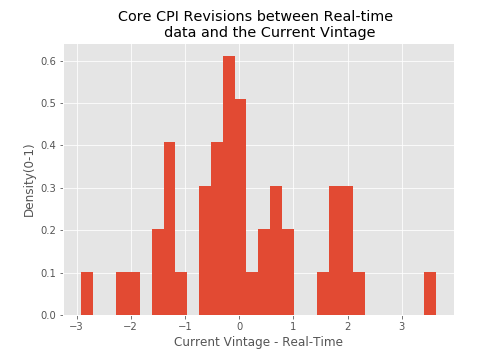
\includegraphics[width=0.7\textwidth]{figures/hist_rev_realtime.png}
\caption{Revisions of Current-vintage from Real-time Core CPI}
\label{real_time_rev}
	\begin{flushleft}
	{\footnotesize Note: real-time data  at time $t$ is defined the inflation from $t-1$ to $t$ according to the most recent vintage of CPI inflation at time $t$. The period is between 2000 M1-2018 M3.}
\end{flushleft}
\end{figure}


\begin{figure}[htbp]
	\centering
	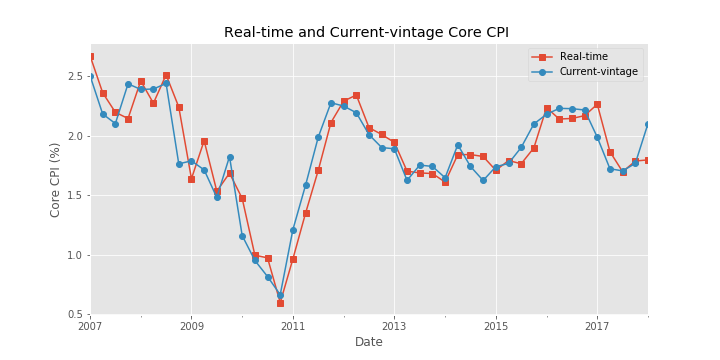
\includegraphics[width=0.8\textwidth]{figures/ts_rev_realtime.png}
	\caption{Current-vintage and Real-time Core CPI}
	\label{ts_real_time_current_vintage}
\end{figure}

\subsection{Results for AR1}

\subsubsection{Professional Forecasters}

Figure \ref{SE_diag_SPF} and \ref{SE_diag_joint_SPF} plot the estimated moments for SE model together with the data moments professional forecasts of SPF. 

From left to the right, the four columns of the figures are based on estimation using different choices of moments. 

Figure \ref{NI_diag_SPF} and \ref{NI_diag_joint_SPF} plot the estimated moments for NI model together with the data moments professional forecasts of SPF. 

\begin{figure}[ht]
	\centering
	\begin{subfigure}[b]{\textwidth}
		\centering
		\caption{Estimation of SE for Professionals}
		\label{SE_diag_SPF}
		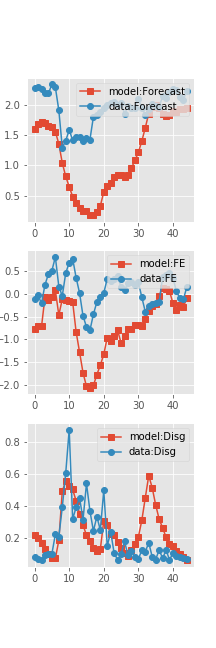
\includegraphics[width=0.19\textwidth]{figures/spf_se_est_diag0.png}
		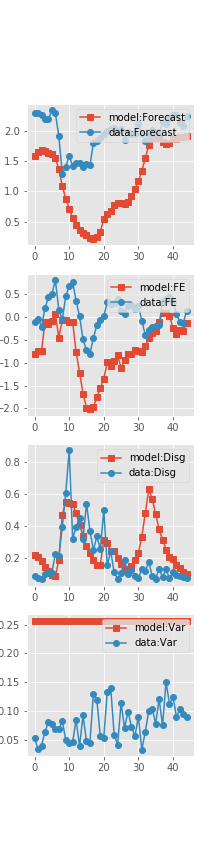
\includegraphics[width=0.19\textwidth]{figures/spf_se_est_diag1.png}
		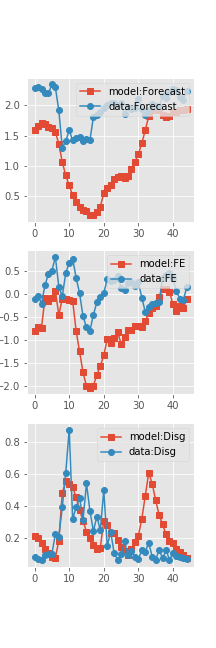
\includegraphics[width=0.19\textwidth]{figures/spf_se_est_diag2.png}
		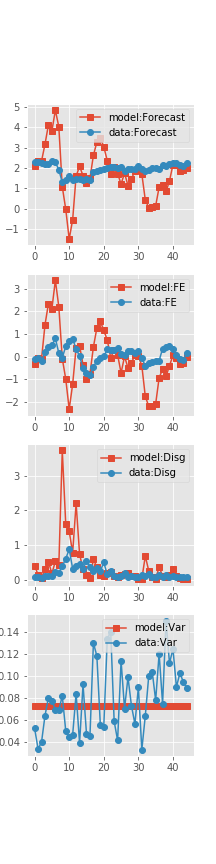
\includegraphics[width=0.19\textwidth]{figures/spf_se_est_diag3.png}
		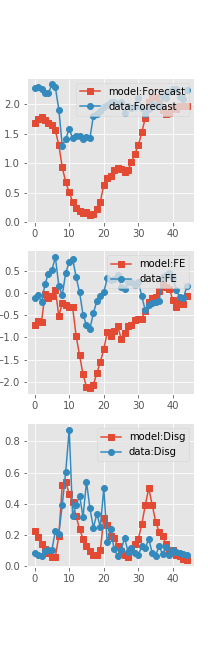
\includegraphics[width=0.19\textwidth]{figures/spf_se_est_diag4.png}
	\end{subfigure}
	\vspace{1em}
	\vfill
	\begin{subfigure}[b]{\textwidth}
		\centering
		\caption{Joint Estimation of SE and Inflation Process}
		\label{SE_diag_joint_SPF}
	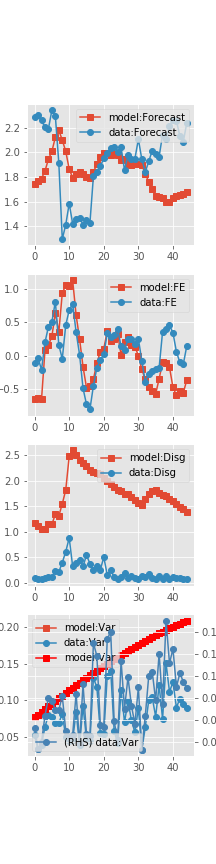
\includegraphics[width=0.19\textwidth]{figures/spf_se_est_joint_diag0.png}
	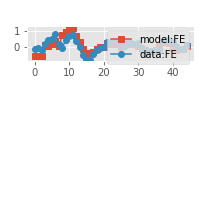
\includegraphics[width=0.19\textwidth]{figures/spf_se_est_joint_diag1.png}
	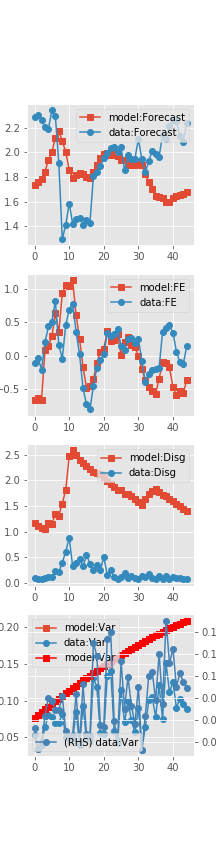
\includegraphics[width=0.19\textwidth]{figures/spf_se_est_joint_diag2.png}
	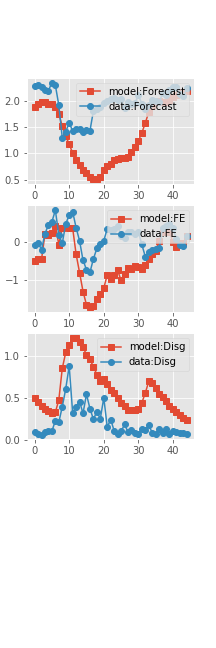
\includegraphics[width=0.19\textwidth]{figures/spf_se_est_joint_diag3.png}
	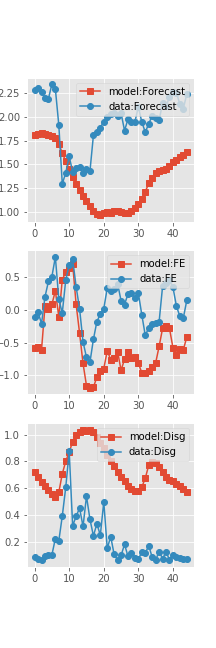
\includegraphics[width=0.19\textwidth]{figures/spf_se_est_joint_diag4.png}
	\end{subfigure}
	\\
	\begin{flushleft}
		{\footnotesize Note: the upper panel estimates expectation formation only taking the process of inflation parameters as given. The bottom panel estimates the parameters of expectation formation and inflation process jointly. From left to the right, the moments used are $\overline y_{t|t}$, $\overline{FE}_{t}$, $\overline y_{t|t}$/$\overline{FE}_{t}$ and $\overline y_{t|t}$ / $\overline{FE}_{t}$/ $\overline{\textrm{Disg}_t}$, $\overline y_{t|t}$ / $\overline{FE}_{t}$/ $\overline{\textrm{Disg}_t}$/$\overline{Var}_t$,  respectively. }
	\end{flushleft}
	\caption{SE of Professionals: Esimated Model Moments and Data Moments}
\end{figure}


\begin{figure}[ht]
	\centering
	\begin{subfigure}[b]{\textwidth}
		\centering
		\caption{Estimation of NI for Professionals}
		\label{NI_diag_SPF}
		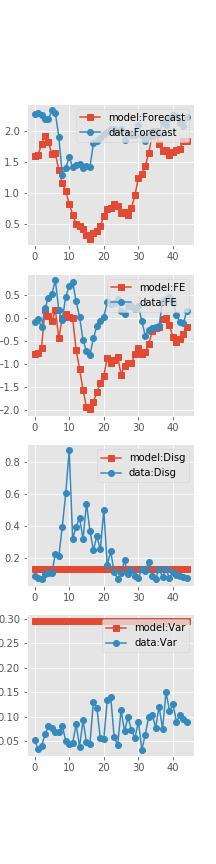
\includegraphics[width=0.19\textwidth]{figures/spf_ni_est_diag0.png}
		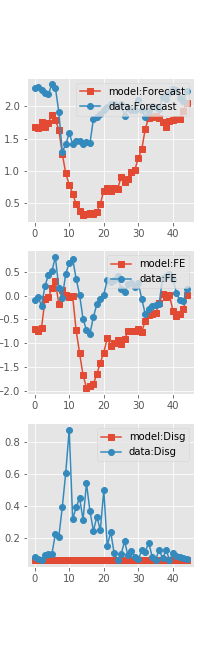
\includegraphics[width=0.19\textwidth]{figures/spf_ni_est_diag1.png}
		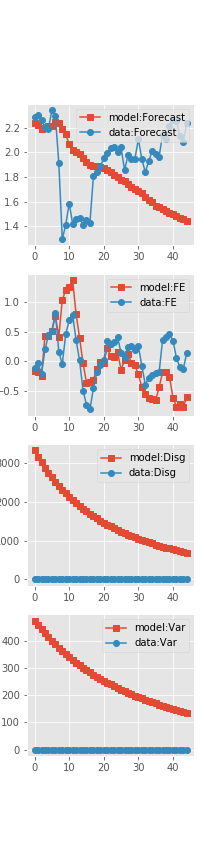
\includegraphics[width=0.19\textwidth]{figures/spf_ni_est_diag2.png}
		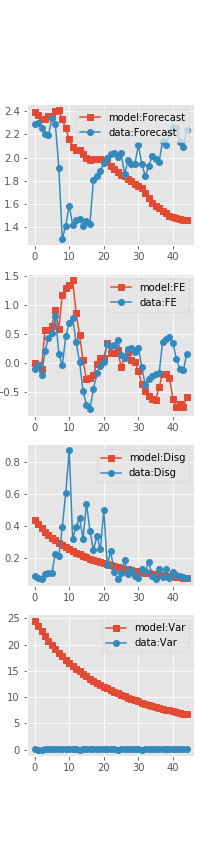
\includegraphics[width=0.19\textwidth]{figures/spf_ni_est_diag3.png}
		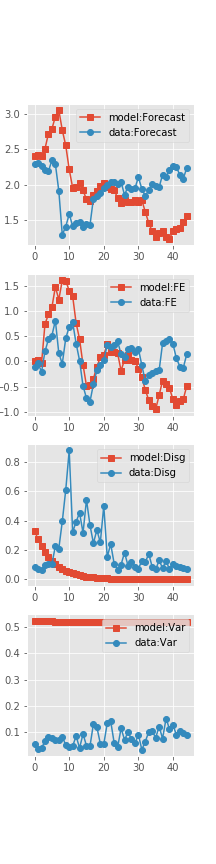
\includegraphics[width=0.19\textwidth]{figures/spf_ni_est_diag4.png}
	\end{subfigure}
	\vspace{1em}
	\vfill
	\begin{subfigure}[b]{\textwidth}
		\centering
		\caption{Joint Estimation of NI and Inflation Process}
		\label{NI_diag_joint_SPF}
		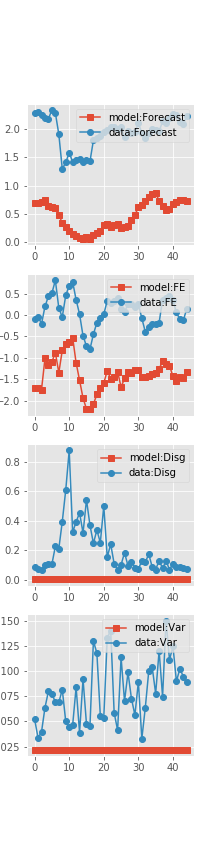
\includegraphics[width=0.19\textwidth]{figures/spf_ni_est_joint_diag0.png}
		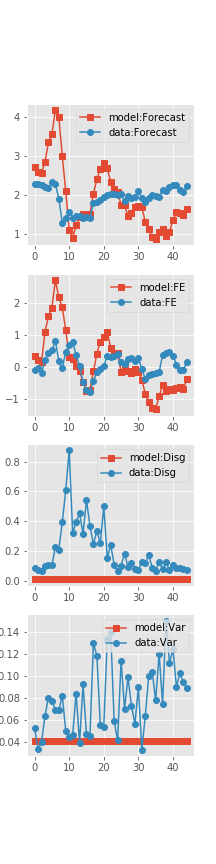
\includegraphics[width=0.19\textwidth]{figures/spf_ni_est_joint_diag1.png}
		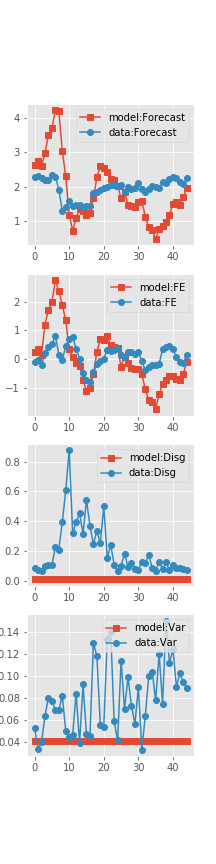
\includegraphics[width=0.19\textwidth]{figures/spf_ni_est_joint_diag2.png}
		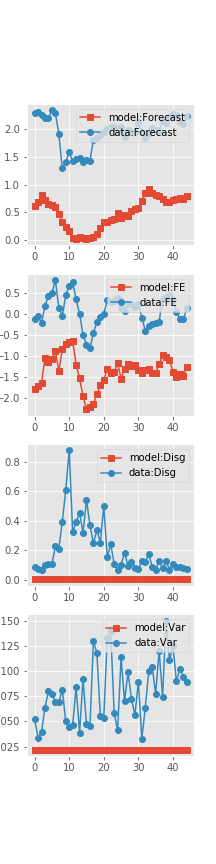
\includegraphics[width=0.19\textwidth]{figures/spf_ni_est_joint_diag3.png}
		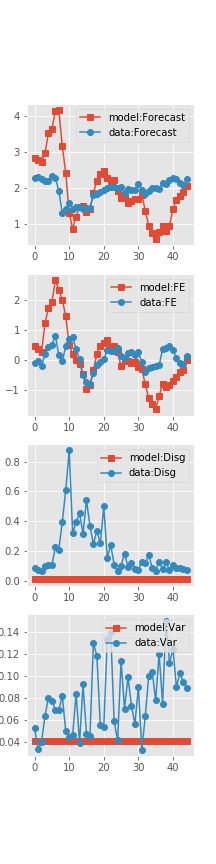
\includegraphics[width=0.19\textwidth]{figures/spf_ni_est_joint_diag4.png}
	\end{subfigure}
	\\
	\begin{flushleft}
		{\footnotesize Note: the upper panel estimates expectation formation only taking the process of inflation parameters as given. The bottom panel estimates the parameters of expectation formation and inflation process jointly. From left to the right, the moments used are $\overline y_{t|t}$, $\overline{FE}_{t}$, $\overline y_{t|t}$/$\overline{FE}_{t}$ and $\overline y_{t|t}$ / $\overline{FE}_{t}$/ $\overline{\textrm{Disg}_t}$, $\overline y_{t|t}$ / $\overline{FE}_{t}$/ $\overline{\textrm{Disg}_t}$/$\overline{Var}_t$,  respectively. }
	\end{flushleft}
	\caption{NI of Professionals: Esimated Model Moments and Data Moments}
\end{figure}


\begin{figure}[ht]
	\centering
	\begin{subfigure}[b]{\textwidth}
		\centering
		\caption{Parameter Learning for Professionals}
		\label{PL_diag_SPF}
		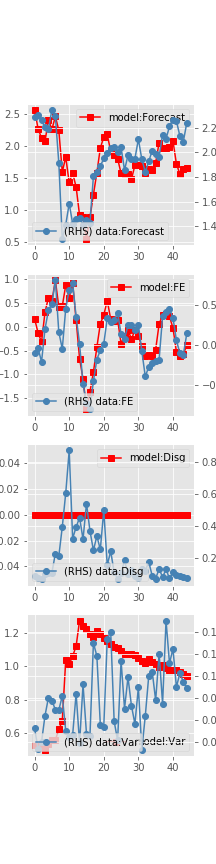
\includegraphics[width=0.19\textwidth]{figures/spf_pl_est_diag.png}
	\end{subfigure} \\
	\begin{flushleft}
		{\footnotesize Note: the figure plots the predicted moments for a prameter learning (PL) model with AR(1) process of inflation.}
	\end{flushleft}
	\caption{PL of Professionals: Esimated Model Moments and Data Moments}
\end{figure}


\subsubsection{Households}


Figure \ref{SE_diag_SCE} and \ref{SE_diag_joint_SCE} plot the estimated moments for SE model together with the data moments of households inflation forecasts from SCE. 

From left to the right, the four columns of the figures are based on estimation using different choices of moments. 

Figure \ref{NI_diag_SCE} and \ref{NI_diag_joint_SCE} plot the estimated moments for NI model together with the data moments of households inflation forecasts from SCE. 

\begin{figure}[htbp]
	\centering
	\begin{subfigure}[b]{\textwidth}
		\centering
		\caption{Estimation of SE for Households}
		\label{SE_diag_SCE}
		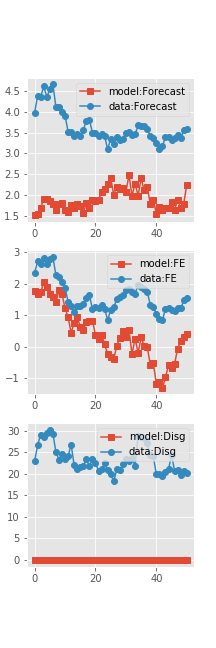
\includegraphics[width=0.19\textwidth]{figures/sce_se_est_diag0.png}
		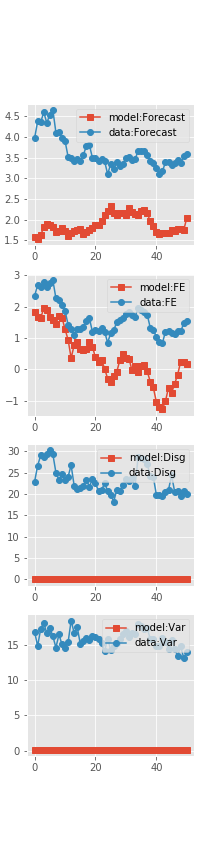
\includegraphics[width=0.19\textwidth]{figures/sce_se_est_diag1.png}
		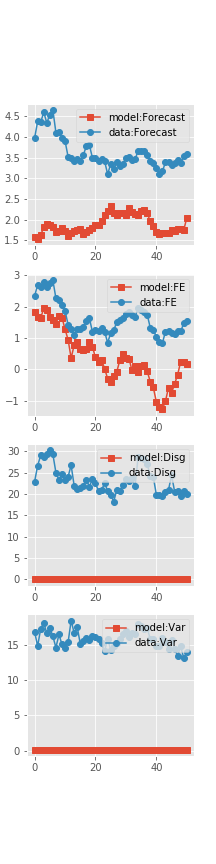
\includegraphics[width=0.19\textwidth]{figures/sce_se_est_diag2.png}
		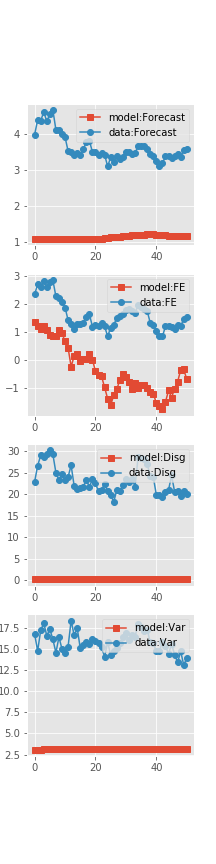
\includegraphics[width=0.19\textwidth]{figures/sce_se_est_diag3.png}
		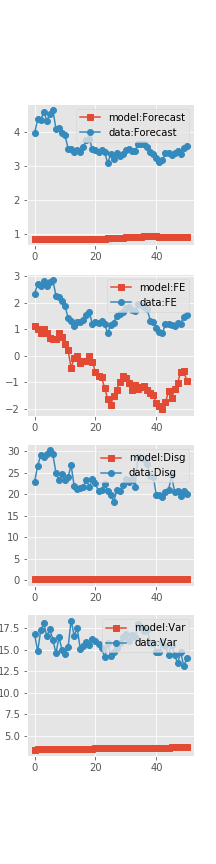
\includegraphics[width=0.19\textwidth]{figures/sce_se_est_diag4.png}
	\end{subfigure}
	\vspace{1em}
	\vfill
	\begin{subfigure}[b]{\textwidth}
		\centering
		\caption{Joint Estimation of SE and Inflation Process}
		\label{SE_diag_joint_SCE}
		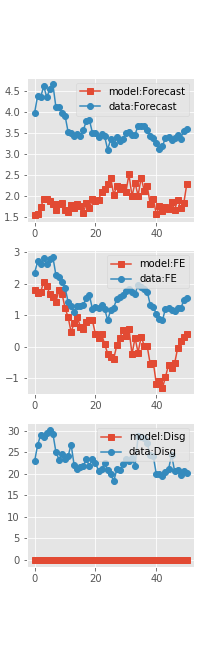
\includegraphics[width=0.19\textwidth]{figures/sce_se_est_joint_diag0.png}
		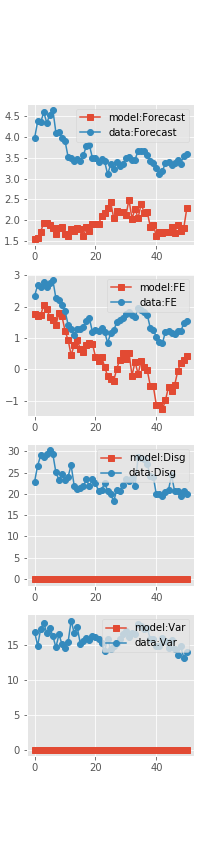
\includegraphics[width=0.19\textwidth]{figures/sce_se_est_joint_diag1.png}
		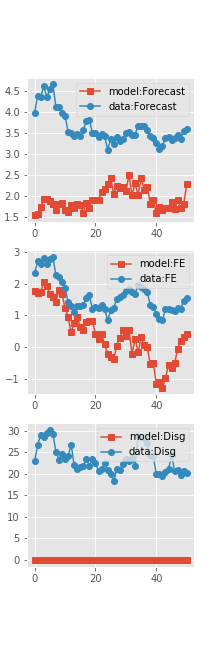
\includegraphics[width=0.19\textwidth]{figures/sce_se_est_joint_diag2.png}
		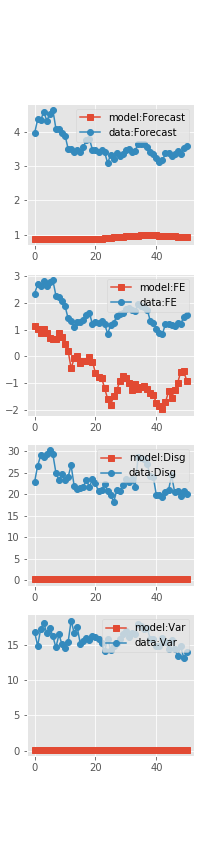
\includegraphics[width=0.19\textwidth]{figures/sce_se_est_joint_diag3.png}
		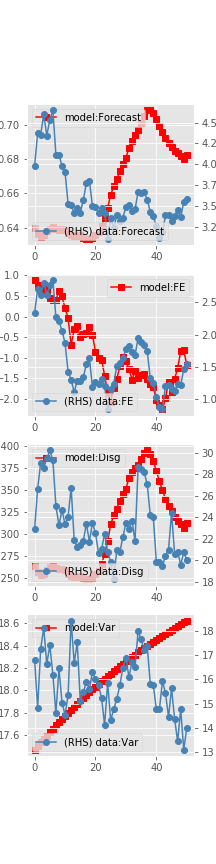
\includegraphics[width=0.19\textwidth]{figures/sce_se_est_joint_diag4.png}
	\end{subfigure}
	\\
	\begin{flushleft}
		{\footnotesize Note: the upper panel estimates expectation formation only taking the process of inflation parameters as given. The bottom panel estimates the parameters of expectation formation and inflation process jointly. From left to the right, the moments used are $\overline y_{t|t}$, $\overline{FE}_{t}$, $\overline y_{t|t}$/$\overline{FE}_{t}$ and $\overline y_{t|t}$ / $\overline{FE}_{t}$/ $\overline{\textrm{Disg}_t}$, $\overline y_{t|t}$ / $\overline{FE}_{t}$/ $\overline{\textrm{Disg}_t}$/$\overline{Var}_t$,  respectively. }
	\end{flushleft}
	\caption{SE of Households: Esimated Model Moments and Data Moments}
\end{figure}


\begin{figure}[htbp]
	\centering
	\begin{subfigure}[b]{\textwidth}
		\centering
		\caption{Estimation of NI  for Households}
		\label{NI_diag_SCE}
		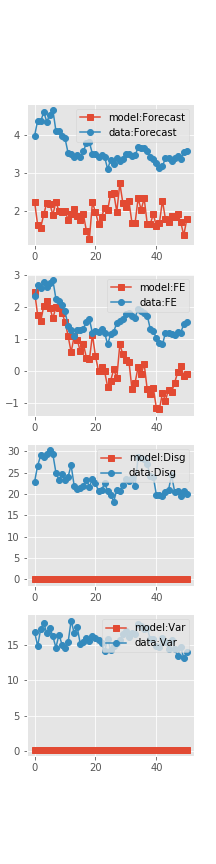
\includegraphics[width=0.19\textwidth]{figures/sce_ni_est_diag0.png}
		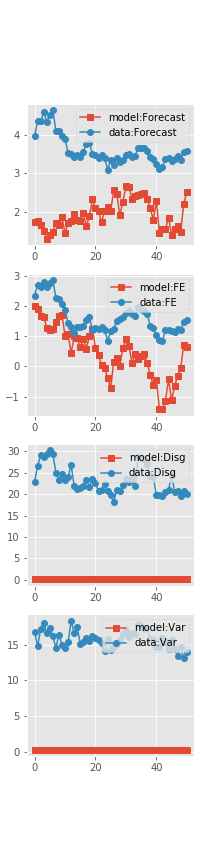
\includegraphics[width=0.19\textwidth]{figures/sce_ni_est_diag1.png}
		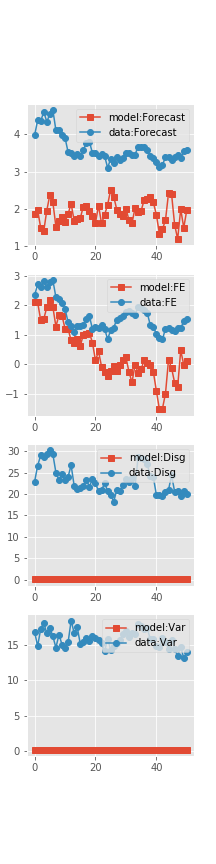
\includegraphics[width=0.19\textwidth]{figures/sce_ni_est_diag2.png}
		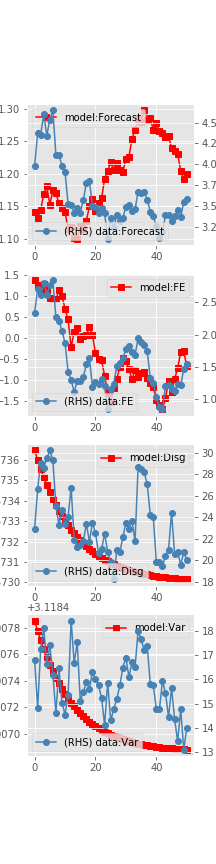
\includegraphics[width=0.19\textwidth]{figures/sce_ni_est_diag3.png}
		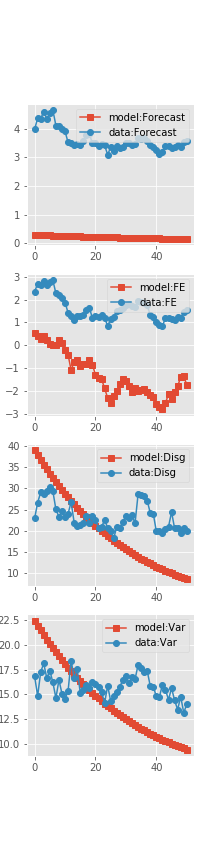
\includegraphics[width=0.19\textwidth]{figures/sce_ni_est_diag4.png}
	\end{subfigure}
	\vspace{1em}
	\vfill
	\begin{subfigure}[b]{\textwidth}
		\centering
		\caption{Joint Estimation of SE and Inflation Process}
		\label{NI_diag_joint_SCE}
		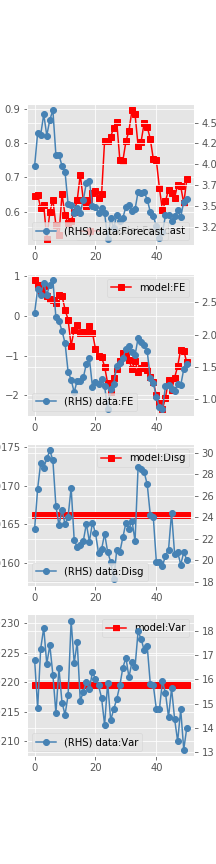
\includegraphics[width=0.19\textwidth]{figures/sce_ni_est_joint_diag0.png}
		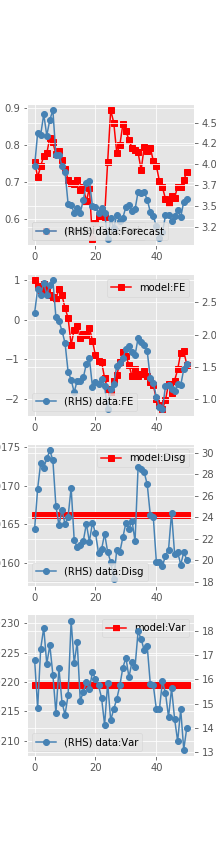
\includegraphics[width=0.19\textwidth]{figures/sce_ni_est_joint_diag1.png}
		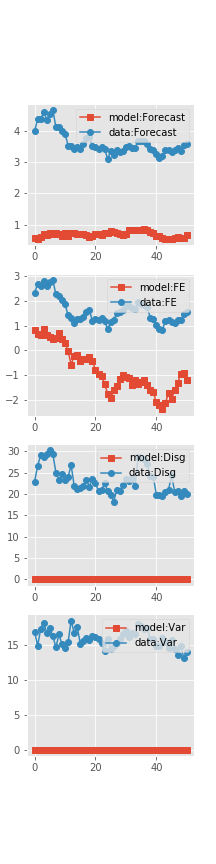
\includegraphics[width=0.19\textwidth]{figures/sce_ni_est_joint_diag2.png}
		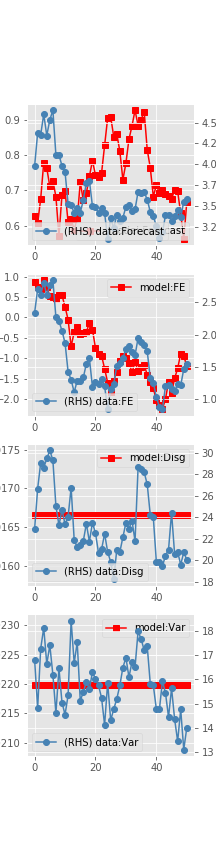
\includegraphics[width=0.19\textwidth]{figures/sce_ni_est_joint_diag3.png}
		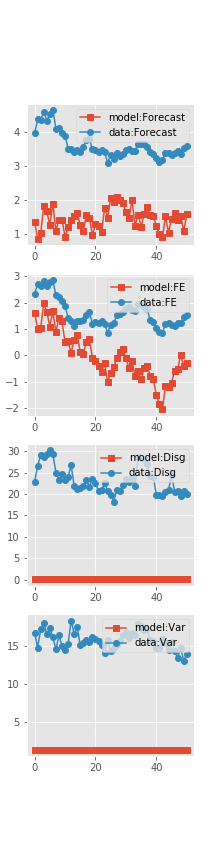
\includegraphics[width=0.19\textwidth]{figures/sce_ni_est_joint_diag4.png}
	\end{subfigure}
	\\
	\begin{flushleft}
		{\footnotesize Note: the upper panel estimates expectation formation only taking the process of inflation parameters as given. The bottom panel estimates the parameters of expectation formation and inflation process jointly. From left to the right, the moments used are $\overline y_{t|t}$, $\overline{FE}_{t}$, $\overline y_{t|t}$/$\overline{FE}_{t}$ and $\overline y_{t|t}$ / $\overline{FE}_{t}$/ $\overline{\textrm{Disg}_t}$, $\overline y_{t|t}$ / $\overline{FE}_{t}$/ $\overline{\textrm{Disg}_t}$/$\overline{Var}_t$,  respectively.  }
	\end{flushleft}
	\caption{NI of Households: Esimated Model Moments and Data Moments}
\end{figure}

	\begin{sidewaystable}[t]
		\centering
	\caption{GMM Estimates of Parameters of SE and Inflation Process}
	\label{GMM_Est_SE_Table}
\begin{tabular}{llllllllllll}
	\hline 
	& 1  & 2    & 3   & SE: $\hat\lambda_{SPF}$(Q) & SE: $\hat\lambda_{SPF}$(Q) & SE: $\rho$ & SE: $\sigma$ & SE: $\hat\lambda_{SCE}$(M) & SE: $\hat\lambda_{SCE}$(M) & SE: $\rho$ & SE: $\sigma$ \\
	\hline 
	Forecast &    &      &     & 0.05                       & 0.03                       & 1          & 0.1          & 1                          & 1                          & 1          & 0.1          \\
	FE       &    &      &     & 0.05                       & 0.03                       & 1          & 0.1          & 1                          & 1                          & 1          & 0.1          \\
	Forecast & FE &      &     & 0.05                       & 0.03                       & 1          & 0.1          & 1                          & 1                          & 1          & 0.1          \\
	Forecast & FE & Disg &     & 0.7                        & 0.38                       & 0.88       & 0.1          & 0.02                       & 0.03                       & 0.98       & 0.1          \\
	Forecast & FE & Disg & Var & 0.7                        & 0.38                       & 0.88       & 0.2          & 0.01                       & 0.03                       & 0.98       & 1.11     \\
	\hline    
\end{tabular}
\end{sidewaystable}


\begin{sidewaystable}[t]
	\centering
	\caption{GMM Estimates of Parameters of NI and Inflation Process}
	\label{GMM_Est_NI_Table}
\begin{tabular}{llllllllllllllll}
	\hline 
	0        & 1   & 2    & 3   & NI: $\hat\sigma_{pb,SPF}$ & $\hat\sigma_{pr,SPF}$ & NI: $\hat\sigma_{pb,SPF}$ & $\hat\sigma_{pr,SPF}$ & NI: $\rho$ & NI: $\sigma$ & NI: $\hat\sigma_{pb,SCE}$ & $\hat\sigma_{pr,SCE}$ & NI: $\hat\sigma_{pb,SCE}$ & $\hat\sigma_{pr,SCE}$ & NI: $\rho$ & NI: $\sigma$ \\
	\hline 
	Forecast &     &      &     & 5.64                      & 804.51                & 0.5                       & 0.5                   & 1          & 0.1          & 93.17                     & 0.64                  & 0.5                       & 0.5                   & 0.8        & 0.1          \\
	FE       &     &      &     & 2197.33                   & 60.45                 & 0.5                       & 0.5                   & 1          & 0.1          & 0.62                      & 0.34                  & 0.5                       & 0.5                   & 0.8        & 0.1          \\
	Forecast & FE  &      &     & 8565.83                   & 176.23                & 0.5                       & 0.5                   & 1          & 0.1          & 0.62                      & 0.44                  & 0.5                       & 0.5                   & 0.8        & 0.1          \\
	Forecast & FE  & Disg &     & 30.39                     & 353.42                & 0.5                       & 0.5                   & 1          & 0.1          & 3154.03                   & 10.93                 & 0.5                       & 0.5                   & 0.8        & 0.1          \\
	Forecast & FE  & Disg & Var & 2.43                      & 63.03                 & 0.5                       & 0.5                   & 1          & 0.1          & 22970.9                   & 332.03                & 0.5                       & 0.5                   & 0.8        & 0.1          \\
	Disg     & Var &      &     & 90.12                     & 0.56                  & 0.5                       & 0.5                   & 1          & 0.1          & 3297.11                   & 333.49                & 0.5                       & 0.5                   & 0.8        & 0.1       \\
	\hline   
\end{tabular}
\end{sidewaystable}


\begin{figure}[ht]
	\centering
	\begin{subfigure}[b]{\textwidth}
		\centering
		\caption{Parameter Learning for Households}
		\label{PL_diag_SCE}
		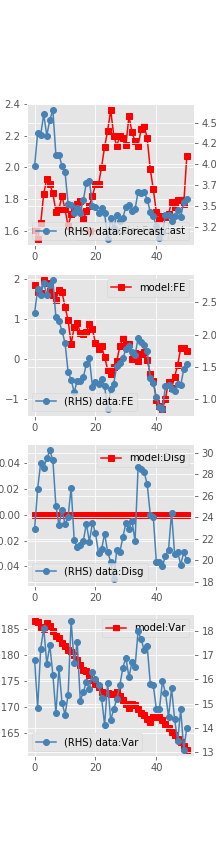
\includegraphics[width=0.19\textwidth]{figures/sce_pl_est_diag.png}
	\end{subfigure} \\
	\begin{flushleft}
		{\footnotesize Note: the figure plots the predicted moments for a prameter learning (PL) model with AR(1) process of inflation.}
	\end{flushleft}
	\caption{PL of Households: Esimated Model Moments and Data Moments}
\end{figure}


\subsection{Results for Stochastic Volatility}

\subsubsection{Professionals Forecasters}


\begin{figure}[ht]
	\centering
	\begin{subfigure}[b]{\textwidth}
		\centering
		\caption{Estimation of SESV for Professionals}
		\label{SESV_diag_SPF}
		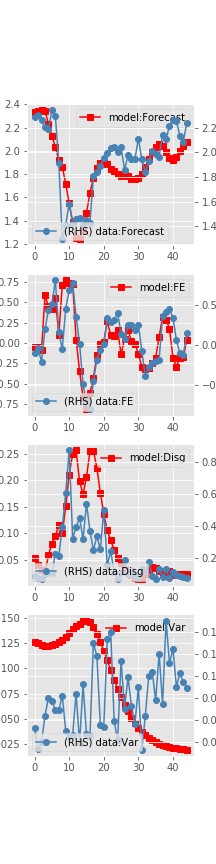
\includegraphics[width=0.19\textwidth]{figures/spf_se_est_sv_diag0.png}
		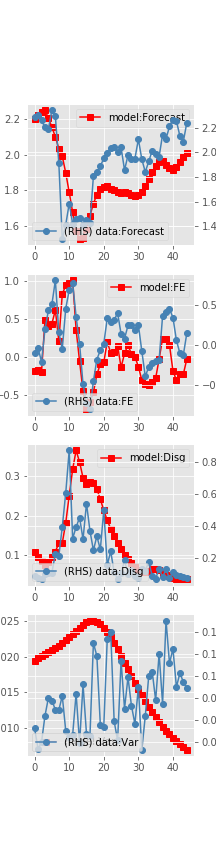
\includegraphics[width=0.19\textwidth]{figures/spf_se_est_sv_diag1.png}
		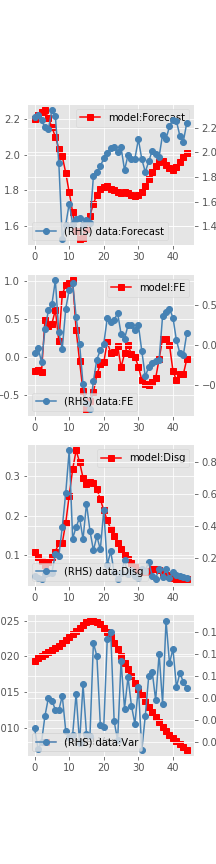
\includegraphics[width=0.19\textwidth]{figures/spf_se_est_sv_diag2.png}
		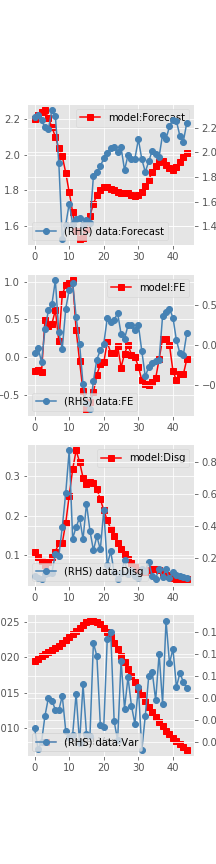
\includegraphics[width=0.19\textwidth]{figures/spf_se_est_sv_diag3.png}
		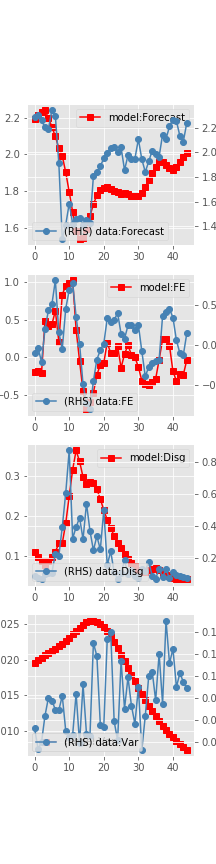
\includegraphics[width=0.19\textwidth]{figures/spf_se_est_sv_diag4.png}
	\end{subfigure}
	\begin{flushleft}
		{\footnotesize Note: this figures plot the data and estimated moments for a  sticky expectation (SE) model with stochastical volatility to inflation. From left to the right, the moments used are $\overline y_{t|t}$, $\overline{FE}_{t}$, $\overline y_{t|t}$/$\overline{FE}_{t}$ and $\overline y_{t|t}$ / $\overline{FE}_{t}$/ $\overline{\textrm{Disg}_t}$, $\overline y_{t|t}$ / $\overline{FE}_{t}$/ $\overline{\textrm{Disg}_t}$/$\overline{Var}_t$,  respectively. }
	\end{flushleft}
	\caption{SESV of Professionals: Esimated Model Moments and Data Moments}
\end{figure}


\begin{figure}[ht]
	\centering
	\begin{subfigure}[b]{\textwidth}
		\centering
		\caption{Estimation of NISV for Professionals}
		\label{NISV_diag_SPF}
		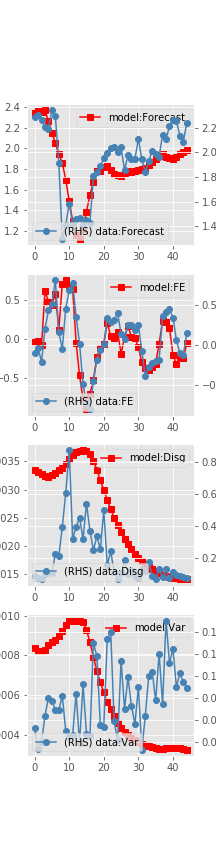
\includegraphics[width=0.19\textwidth]{figures/spf_ni_est_sv_diag0.png}
		\includegraphics[width=0.19\textwidth]{figures/spf_ni_est_sv_diag1.png}
		\includegraphics[width=0.19\textwidth]{figures/spf_ni_est_sv_diag2.png}
		\includegraphics[width=0.19\textwidth]{figures/spf_ni_est_sv_diag3.png}
		\includegraphics[width=0.19\textwidth]{figures/spf_ni_est_sv_diag4.png}
	\end{subfigure}
	\begin{flushleft}
		{\footnotesize Note: this figures plot the data and estimated moments for a noisy information (NI) model  with stochastical volatility to inflation. From left to the right, the moments used are $\overline y_{t|t}$, $\overline{FE}_{t}$, $\overline y_{t|t}$/$\overline{FE}_{t}$ and $\overline y_{t|t}$ / $\overline{FE}_{t}$/ $\overline{\textrm{Disg}_t}$, $\overline y_{t|t}$ / $\overline{FE}_{t}$/ $\overline{\textrm{Disg}_t}$/$\overline{Var}_t$,  respectively. }
	\end{flushleft}
	\caption{NISV of Professionals: Esimated Model Moments and Data Moments}
\end{figure}


\subsubsection{Households}


\begin{figure}[ht]
	\centering
	\begin{subfigure}[b]{\textwidth}
		\centering
		\caption{Estimation of SESV for Households}
		\label{SESV_diag_SCE}
		\includegraphics[width=0.19\textwidth]{figures/sce_se_est_sv_diag0.png}
		\includegraphics[width=0.19\textwidth]{figures/sce_se_est_sv_diag1.png}
		\includegraphics[width=0.19\textwidth]{figures/sce_se_est_sv_diag2.png}
		\includegraphics[width=0.19\textwidth]{figures/sce_se_est_sv_diag3.png}
		\includegraphics[width=0.19\textwidth]{figures/sce_se_est_sv_diag4.png}
	\end{subfigure}
	\begin{flushleft}
		{\footnotesize Note: this figures plot the data and estimated moments for a  sticky expectation (SE) model with stochastical volatility to inflation. From left to the right, the moments used are $\overline y_{t|t}$, $\overline{FE}_{t}$, $\overline y_{t|t}$/$\overline{FE}_{t}$ and $\overline y_{t|t}$ / $\overline{FE}_{t}$/ $\overline{\textrm{Disg}_t}$, $\overline y_{t|t}$ / $\overline{FE}_{t}$/ $\overline{\textrm{Disg}_t}$/$\overline{Var}_t$,  respectively. }
	\end{flushleft}
	\caption{SESV of Households: Esimated Model Moments and Data Moments}
\end{figure}


\begin{figure}[ht]
	\centering
	\begin{subfigure}[b]{\textwidth}
		\centering
		\caption{Estimation of NISV for Households}
		\label{NISV_diag_SCE}
		\includegraphics[width=0.19\textwidth]{figures/sce_ni_est_sv_diag0.png}
		\includegraphics[width=0.19\textwidth]{figures/sce_ni_est_sv_diag1.png}
		\includegraphics[width=0.19\textwidth]{figures/sce_ni_est_sv_diag2.png}
		\includegraphics[width=0.19\textwidth]{figures/sce_ni_est_sv_diag3.png}
		\includegraphics[width=0.19\textwidth]{figures/sce_ni_est_sv_diag4.png}
	\end{subfigure}
	\begin{flushleft}
		{\footnotesize Note: this figure plots the data and estimated moments for a noisy information (NI) model  with stochastical volatility to inflation. From left to the right, the moments used are $\overline y_{t|t}$, $\overline{FE}_{t}$, $\overline y_{t|t}$/$\overline{FE}_{t}$ and $\overline y_{t|t}$ / $\overline{FE}_{t}$/ $\overline{\textrm{Disg}_t}$, $\overline y_{t|t}$ / $\overline{FE}_{t}$/ $\overline{\textrm{Disg}_t}$/$\overline{Var}_t$,  respectively. }
	\end{flushleft}
	\caption{NISV of Households: Esimated Model Moments and Data Moments}
\end{figure}


\begin{sidewaystable}[t]
	\centering
	\caption{GMM Estimates of Parameters of SESV}
	\label{GMM_Est_SE_SV_Table}
	\begin{tabular}{llllll}
		\hline 
		0        & 1  & 2    & 3   & SE: $\hat\lambda_{SPF}$(Q) & SE: $\hat\lambda_{SCE}$(M) \\
		\hline 
		Forecast &    &      &     & 0.23                       & 0.01                       \\
		FE       &    &      &     & 0.12                       & 1                          \\
		Forecast & FE &      &     & 0.12                       & 1                          \\
		Forecast & FE & Disg &     & 0.12                       & 1                          \\
		Forecast & FE & Disg & Var & 0.12                       & 1           \\
		\hline               
	\end{tabular}
\end{sidewaystable}


\begin{sidewaystable}[t]
	\centering
	\caption{GMM Estimates of Parameters of NISV}
	\label{GMM_Est_NI_SV_Table}
\begin{tabular}{llllllllllllll}
		\hline 
	0        & 1  & 2    & 3   & NI: $\hat\sigma_{pb,SPF}$ & $\hat\sigma_{pr,SPF}$ & $Var$ & $y$ & Disg & NI: $\hat\sigma_{pb,SCE}$ & $\hat\sigma_{pr,SCE}$ & $Var$ & $y$ & Disg \\
	\hline 
	Forecast &    &      &     & 0.05                      & 0.02                  & 0.54  & 1   & 5    & 12.09                     & 12.16                 & 0     & 1   & 2    \\
	FE       &    &      &     & 0                         & 0.27                  & 1.06  & 1   & 5    & 130.13                    & 764.51                & 30.99 & 1   & 2    \\
	Forecast & FE &      &     & 0.16                      & 0                     & 1.06  & 1   & 5    & 168.48                    & 695.91                & 43.31 & 1   & 2    \\
	Forecast & FE & Disg &     & 0                         & 0.22                  & 1.06  & 1   & 5    & 166.89                    & 6.1                   & 0.03  & 1   & 2    \\
	Forecast & FE & Disg & Var & 0                         & 0.24                  & 1.07  & 1   & 5    & 362.11                    & 6.26                  & 0.04  & 1   & 2   \\
	\hline 
\end{tabular}
\end{sidewaystable}



\end{document}
